\documentclass[a4paper,amsmath]{oblivoir}

\usepackage{fapapersize}
\usefapapersize{*,*,1in,*,1in,*}

\makeatletter
\let\ATonum\@onum
\makeatother

\usepackage{xcolor}
\usepackage{graphicx}
\usepackage{hologo}
\usepackage{relsize}
\usepackage{tcolorbox}
\tcbuselibrary{listings,breakable}
\tcbset{listing engine=listings,colframe=cyan,colback=cyan!5!white}

\setmainfont{Noto Serif}
\setsansfont{Noto Sans}
\setmonofont{Noto Sans Mono}
\setkomainfont(Noto Serif CJK KR)(* Bold)(Noto Sans CJK KR)
\setkosansfont[Noto Sans CJK KR]()( Bold)( Medium)
\usepackage{unicode-math}
\setmathfont{LibertinusMath-Regular.otf}

\newcounter{sub}
\newcommand\bangotsuite{\stepcounter{sub}\thesub}

\setlength{\parindent}{0mm}

\newcommand\pkg[1]{\textsf{#1}}

\ExplSyntaxOn 

\NewDocumentEnvironment {intro} {o}
{
    \IfValueTF { #1 }
    {
        \int_set:Nn \l_tmpa_int { #1 }
    }
    {
        \int_set:Nn \l_tmpa_int { 1 }
    }
    \noindent \rule {\linewidth}{3pt}
    \par 
    \sffamily [No.\space\int_use:N \l_tmpa_int ]\ \ 
    \bfseries
}
{
    \hfill \underline{\hphantom{2019}}년~\underline{\hphantom{06}}월~ \underline{\hphantom{25}}일 
    \par 
    \vskip -.3\baselineskip 
    \noindent \rule {\linewidth }{1pt}
    \par 
    \vskip .5\baselineskip 
}

\NewDocumentCommand \exverb { d|| }
{
	\texttt { \tl_to_str:n { #1 } }
}

\ExplSyntaxOff 

\NewDocumentEnvironment {questiona} { m }
{
%	\medskip
	\begin{tcolorbox}[title={#1},fonttitle={\sffamily\bfseries}]
}{%
	\end{tcolorbox}
}

\NewDocumentEnvironment {questionp} { }
{
%	\medskip
	\begin{tcolorbox}[colframe=orange!30!black!60,colbacktitle=orange!25!gray,
	title={연습문제},fonttitle={\sffamily\bfseries}]
}{%
	\end{tcolorbox}
}


\NewDocumentEnvironment {exampleonly} {}
{%
%	\begin{tcblisting}{listing only}
	\expandafter\tcblisting{listing only,breakable,before={\par\medskip\setstretch{1}}}
}{
	\endtcblisting
%	\end{tcblisting}
}

\NewDocumentEnvironment {exampleside} {}
{%
	\tcblisting{listing side text,breakable,before={\par\medskip\setstretch{1}}}%
}{%
	\endtcblisting
}

%\NewDocumentEnvironment {examplebelow} {}
%{%
%	\medskip
%	\tcblisting{text below listing,breakable}%
%}{%
%	\endtcblisting
%}
\newtcblisting{examplebelow}{breakable,before={\par\medskip\setstretch{1}}}

\begin{document}

\begin{intro}[3]
Merry-Go-Round
\end{intro}

\begin{questiona}{문제}
$1$부터 입력받은 정수(자연수)까지의 합을 출력하여라.
\tcblower
입력: \verb|\summation{10}|\\
출력: $\displaystyle\sum_{k=1}^{10} = 55$
\end{questiona}

$n$까지의 합을 구하는 것은
\[
\sum_{k=1}^{n} = \frac{n(n+1)}{2}
\]
로 간단히 처리할 수 있다. 
\begin{exampleside}
\ExplSyntaxOn
\NewDocumentCommand \simplesum { m }
{
    \int_eval:n { #1 * (#1+1) / 2 } 
}
\ExplSyntaxOff

\simplesum{10}
\end{exampleside}
나누기가 있는데 정수형으로 반환해도 괜찮을까? 물론 괜찮다. 이유는 $n(n+1)$ 둘 중 하나는 반드시 짝수일 것이기 때문이다.
만약 정수 아닌 결과가 예상되는 경우이고 반드시 정수형으로 값을 내어야 하며 나눗셈이 포함된 식이라면 \verb|\int_eval:n|의 결과가 정수이기는 하겠지만 반올림한 결과일 것이라는 점을 염두에 두어야 할 때가 있을 수 있다.

\section{함수와 프로시저}

Pascal에서는 function과 procedure를 구별한다. \verb|return|이 있는, 즉 어떤 값을 반환하는 것은 function이고 반환값 없이 일정한 처리만을 하는 것이 procedure이다.

expl3의 함수(\textsf{cs})들은 \emph{근본적으로} procedure이다. 그러나 그 “처리”가 입력 스트림에 무엇인가를 남기는 것이라면 그것을 반환값처럼 활용할 수는 있다.
어떤 사용자 정의 함수가 반환값을 가지고 있다고 하더라도 그것이 다른 함수의 인자로 들어가서 확장될 수 있느냐는 또 다른 문제이다. 그래서 expl3 코딩에서는 가능하면 변수 조작을 통해서 문제를 해결하는 것이 복잡한 확장 문제를 피해가기 더 나을 때가 있다.

\begin{examplebelow}
\ExplSyntaxOn
\int_new:N \g_totalsum_int

\NewDocumentCommand \simplesum { m }
{
    \int_gzero:N \g_totalsum_int
    \calc_sum:n { #1 }
    \int_use:N \g_totalsum_int
}

\cs_new:Npn \calc_sum:n #1
{
    \int_gset:Nn \g_totalsum_int { #1 * ( #1 + 1 ) /2 }
}
\ExplSyntaxOff

\simplesum{10}
\end{examplebelow}

이 예시에서 \verb|\calc_sum:n|은 그 자체로 아무 것도 반환하지 않는다. 그 대신 \verb|\g_totalsum_int|라는 전역 변수의 값을 조작하는 “처리”를 행하고 있다.

\subsection*{확장 (2): 인자의 한 번 확장}

이 둘의 차이를 조금 더 살펴보자.

다음 보기를 잘 보아라. 여기서 정의된 \verb|\fn_sum:n|은 “함수”처럼 정의한 것이다.
그러므로 일정한 값을 “반환”할 것이고, 따라서 \verb|\fn_sum:n {\fn_sum:n { 5 } }|라고 명령하면 \verb|\fn_sum:n{15}|의 효과가 나타나야 한다.


\begin{examplebelow}
\ExplSyntaxOn
\cs_new:Npn \fn_sum:n #1
{
    \int_eval:n { #1 * ( #1 + 1 ) / 2 }
}

\exp_args:No \fn_sum:n { \fn_sum:n { 5 } } ~=~ \fn_sum:n { 15 }
\ExplSyntaxOff
\end{examplebelow}


그런데, 잘 생각해보면 \verb|\fn_sum:n|은 숫자가 인자로 들어올 것을 예상하고 있다. 그러므로 인자에 들어가는 것을 확장해주지 않으면 안 된다. 이것은
\begin{verbatim}
\expandafter \fn_sum:n \expandafter { \fn_sum:n { 5 } }
\end{verbatim}
와 같이 해야 할 것인데, expl3에는 인자를 확장하는 손쉬운 방법이 많이 제공된다. 인자를 확장하는  \verb|\exp_args:|라는 (인자형에 따라 여러 가지 variant가 있는) 함수를 알아두자. 이를 이용하여 여러 번 \verb|\expandafter|를 붙여야 하는 불편을 거의 피해갈 수 있다.

\verb|\exp_args:No|에서 N 하나와 o 하나를 지정하였는데 여기서 확장되는 것은 두 번째 인자 o이다. o는 중괄호로 전달되는 그 안의 것을 “한 번”(\textit{o}nce) 확장한다는 의미이다. 
따라서 다음과 같이 쓸 수 있다. (이 자리에서는 \verb|:Nx|로 해도 같은 결과이다. o와 x의 차이에 대해서는 다음에 토론할 기회가 있을 것이다.)
\begin{verbatim}
\exp_args:No \fn_sum:n { \fn_sum:n { 5 } }
\end{verbatim}

그러면 \verb|\tl_set:No \l_a_tl { a }|라는 형식의 명령은 
\begin{verbatim}
\exp_args:NNo \tl_set:Nn \l_a_tl { a }
\end{verbatim}
이것과 동일한 의미임을 알수 있겠다. 항상 n이 기본적인 형태이고 o가 그 확장형임을 기억해두자.

코딩의 가독성과 간결성을 위해서 \verb|\exp_args:|는 남용하지 않는 것이 좋다. 그러나 확장이 문제로 될 때는 당연히 써야 한다. 확장 문제는 앞으로 지속적으로 새로운 형태를 배워가게 된다.

\medskip

\hangfrom{붙임 \bangotsuite: }\textsf{xparse}의 \verb|\NewDocumentCommand|는 기본적으로 protected 명령을 만든다. 그렇기 때문에 이렇게 정의된 명령을 확장하려면 더 깊은 확장 단계를 지시해야 한다. 즉시 확장 가능한 명령을 만드는 \verb|\NewExpandableDocumentCommand|가 있지만 뭔가 길고 불편하다.

\hangfrom{붙임 \bangotsuite: }expl3를 쓰는 한, 인자형에 대해서 규칙을 지켜주는 것이 좋다. 나중에 틀림없이 헷갈리는 날이 온다. 예를 들어 \verb|\int_mod:nn \l_tmpa_int 3|과 같은 코드는 비록 실행이 된다고 하더라도 혼란스럽다. 왜냐하면 n은 “중괄호 범위”로 전달되는 것으로 약속했기 때문이다.
\verb|\my_func:n \l_tmpa_tl|\allowbreak 이 처음에는 좋은 듯하지만 이제 배운 “확장”이 문제가 되면 이것을 o확장해야 할지 V확장해야 할지 틀림없이 헷갈리는 날이 오는 것이다.
번거롭더라도 o확장을 의도한다면 \verb|{ \l_tmpa_int } {3}|\allowbreak 으로 적도록 습관을 들여야 한다. 굳이 위와 같이 간결하게 쓰고 싶다면, \verb|\int_mod:VN|과 같은 형식으로 써두어야 나중에 헷갈리지 않는다. (그런 함수가 제공되지 않는다는 것은 일단 논외로 하고.)

\section{반복문}

이것만으로는 공부가 되기에 부족하므로, 다음과 같은 방법으로 합을 구해보고자 한다.

\medskip

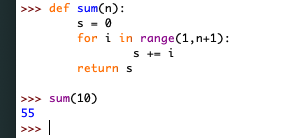
\includegraphics[scale=.9]{screenshot-idle}

expl3의 정수형(\textsf{int})은 부호있는 32비트 정수(signed (long)int)이다. (8비트 CPU 시절에는 이것이 long이었다.) 표현범위는 
\ExplSyntaxOn
$-2^{31}\, (\fp_eval:n { -2^31 })$부터~
$2^{31}-1\, (\fp_eval:n { 2^31 -1 })$
\ExplSyntaxOff
까지이다. 
\verb|\int_eval:n|의 결과가 이 범위를 벗어나면 \texttt{Arithmetic overflow}라는 에러를 보이고 동작을 멈춘다.

\medskip

\hangfrom{붙임 \bangotsuite: }int는 \TeX 의 count를 \hologo{eTeX}이 확장한 것이다. \hologo{eTeX}의 \verb|\numexpr|가 정수 표현식의 출발점이다. 예를 들면 \verb|\int_eval:n { a/b }|가 truncate가 아니라 round인 것도 \hologo{eTeX}으로부터 시작된 것이다. expl3의 정수는 \hologo{eTeX} 엔진에 전적으로 의존한다.

\hangfrom{붙임 \bangotsuite: }32비트를 넘는 큰 수에 대해서 다루려면 \textsf{xint} 엔진을 이용할 수 있는데 이에 대해서
다음 강좌에서 간단히 취급할 생각이다.

\subsection{for loop}

for-loop는 카운터 인덱스가 있는 반복문이다.

표준적인 for-loop 문의 형식
\begin{verbatim}
for i := a to b step c
...
endfor
\end{verbatim}
에서 $i$는 인덱스 카운터이고 $a$는 first, $b$는 last, $c$는 step이다. expl3에는 다음 함수들이 이 역할을 한다.
\begin{itemize} \firmlist
\item \verb|\int_step_function:nN|\quad 1부터 주어지는 수까지 N을 반복. start는 $1$이고 step도 $1$. last가 첫 번째 인자 n이다. 반복할 함수는 N으로 주어진다. 함수가 별도로 정의되지 않고 inline으로 처리할 때 \verb|\int_step_inline:nn|을 쓴다. 인덱스 카운터가 \verb|#1|(다른 함수 정의 내부의 inline 함수라면 \verb|##1|)이다.
\item \verb|\int_step_function:nnN|\quad 시작 숫자가 1일 아닐 때. 첫 번째 n이 start, 두 번째 n이 last이다. 마찬가지로 인덱스는 \verb|#1|이며 inline 함수는 \verb|\int_step_inline:nnn| 꼴로 쓴다.
\item \verb|\int_step_function:nnnN|\quad step이 $1$이 아닐 때. 차례로 start, step, last 순이다. (start, last, step이 아니므로 순서에 주의). 마찬가지로 \verb|\int_step_inline:nnnn|이 있다.
\end{itemize}

간단한 예를 들어두자.
\begin{exampleside}
\ExplSyntaxOn
\int_step_inline:nn { 5 } { #1 \quad } \par
\int_step_inline:nnn { 2 } { 6 } { #1 \quad } \par
\int_step_inline:nnnn { 3 } { 2 } { 11 } { #1 \quad }
\ExplSyntaxOff
\end{exampleside}

다른 범용언어의 for 문과 비교하자면, 숫자를 인덱스로 하는 for-문은 \verb|\int_step_...|과 유사하고 리스트를 인덱스로 하는 for-문은 이미 배운 바 \verb|\..._map_...|과 비슷하다.
단, \verb|\int_step_...| 함수들은 루프 중에 중단할 수 없다. (루프의 탈출이 중요하다면 \verb|step| 함수를 쓰지 말고 \verb|map| 함수를 사용하도록 하라.)

이를 이용하여 앞서 예시한 알고리즘을 expl3로 쓰면,

\begin{examplebelow}
\ExplSyntaxOn
\int_new:N \g_sum_int

\NewDocumentCommand \suma { m }
{
    \int_gzero:N \g_sum_int
    \summation_fn:n { #1 }
    \int_use:N \g_sum_int
}

\cs_new:Npn \summation_fn:n #1
{
    \int_step_inline:nn { #1 }
    {
        \int_gadd:Nn \g_sum_int { ##1 }
    }
}
\ExplSyntaxOff

\suma{100}
\end{examplebelow}


\subsection{while, until}

for를 쓰지 않고 while 반복문으로 같은 일을 할 수 있다.
\begin{tcblisting}{listing only,listing options={language=Python},before={\par\medskip\setstretch{1}}}
def suma(n):
    a=0
    s=0
    while a<n:
        a+=1
        s+=a
    return s
\end{tcblisting}

expl3에서 while형 반복문은 다음 네 가지 형태가 있다.
\begin{enumerate}[(1)] \firmlist
\item \verb|..._while_do:nn|
\item \verb|..._do_while:nn|
\item \verb|..._until_do:nn|
\item \verb|..._do_until:nn|
\end{enumerate}

의미는 직관적으로 이해가 될 것이다. 이 함수의 첫 인자 n은 실은 boolean 값을 반환하는 비교연산식으로 이루어진다. 그러므로 이 함수 형식의 원형은
\begin{verbatim}
\bool_while_do:nn { <bool expr> }
{ ... }
\end{verbatim}
이러한 것이다. \texttt{<bool expr>} 부분에 예컨대 하나의 boolean 변수가 온다고 가정하자.

\begin{examplebelow}
\ExplSyntaxOn
\bool_set_true:N \l_tmpa_bool
\int_zero:N \l_tmpa_int
\bool_while_do:nn { \l_tmpa_bool }
{
    \int_incr:N \l_tmpa_int
    \int_compare:nTF { \l_tmpa_int > 10 }
    {
        \bool_set_false:N \l_tmpa_bool
    }
    {
        a\int_use:N \l_tmpa_int 
        \quad
        \bool_set_true:N \l_tmpa_bool
    }
}
\ExplSyntaxOff
\end{examplebelow}

\paragraph{bool 연산식과 자료형}

bool 연산식은 다음 연산자로 이루어진다. \verb|&&| (and), \verb+||+ (or), \verb|!| (not)과 괄호(\verb|()|).

이제 정수형 데이터에 대하여 while을 어떻게 적용할 것인가를 생각하자. \verb|\l_tmpa_int| 값이 10보다 작으면 true, 그렇지 않으면 false가 되도록 하고 inline function을 true 조건의 while 반복문을 걸어보기로 한다.

\begin{examplebelow}
\ExplSyntaxOn
\int_zero:N \l_tmpa_int

\bool_while_do:nn { \int_compare_p:n { \l_tmpa_int < 10 } }
{
    \int_incr:N \l_tmpa_int
    \int_to_Alph:n { \l_tmpa_int }
}
\ExplSyntaxOff
\end{examplebelow}

\verb|..._p|가 붙는 함수는 boolean 값을 반환한다. 앞서 배운 \verb|\int_compare:nTF|는 사실
\begin{verbatim}
\bool_if:nTF { \int_compare_p:n { ... } }
{ <T> } { <F> }
\end{verbatim}
를 축약한 꼴이다. 이런 종류의 함수로 예컨대 \verb|\tl_if_eq_p:NN|이 있는데 이것은 boolean값을 반환하므로 
\begin{verbatim}
\bool_if:nTF { \tl_if_eq_p:NN <N> <N> } { <T> } { <F> }
\end{verbatim}
라고 쓸 수 있는데 이를 간단히 \verb|\tl_if_eq:NNTF|로 쓸 수 있는 것이다.

이제 \verb|\bool_while_do:nn| \verb|{ \int_compare_p:n| \verb|{ ... } } |이라고 써야 할 것을 간단히 \\
\verb|\int_while_do:nn| \\
으로 쓸 수 있음을 알게 되었다.

그리하여, 각 자료형에 대하여 while 함수가 여러 개 정의된 것처럼 보인다. 실은 \verb|\bool_while_do:nn|의 첫 인자로 각 자료형의 bool 반환 함수를 쓰는 것을 줄여쓰게 한 것인데, 이들을 이런 식으로 설명하는 이유는 두 가지 이상의 조건을 and 또는 or 연산하려면 \verb|\bool_while_do:nn|을 쓸 수 밖에 없기 때문이다. 즉, ``임의의 수가 10보다 크다면 TF하라''는 명령은
\begin{verbatim}
\int_compare:nTF { \l_tmpa_int > 10 } { <T> } { <F> }
\end{verbatim}
로 쓸 수 있지만, $a$가 10보다 크고 $b$가 100보다 작으면이라는 조건은
\begin{verbatim}
\bool_if:nTF 
{
  \int_compare_p:n { \l_tmpa_int > 10 } 
    &&
  \int_compare_p:n { \l_tmpb_int < 100 } 
}
{ <T> } { <F> }
\end{verbatim}
으로 써야 하는데 이에 대한 감각을 익혀두라는 의미이다.

아무튼 각 자료형 별로 while do 형식의 함수를 대강 보면 
\begin{verbatim}
\dim_while_do:nn   \dim_do_while:nn   \dim_until_do:nn   \dim_do_until:nn
\fp_while_do:nn    \fp_do_while:nn    \fp_until_do:nn    \fp_do_until:nn
\int_while_do:nn   \int_do_while:nn   \int_until_do:nn   \int_do_until:nn
\end{verbatim}
등이 있는 것이다.

bool 자료형(\textsf{l3bool})이 변수로서 사용될 수 있다. 이 경우에는 
\begin{verbatim}
\bool_while_do:Nn
\end{verbatim}
을 쓸 수 있는데 \texttt{N} 위치에 임의의 boolean 변수(\verb|\l_tmpa_bool|)가 올 수 있다.
참고로 bool 자료형에서 값을 할당할 적에는
\begin{verbatim}
\bool_set_true:N,    \bool_set_false:N,    \bool_set_inverse:N
\end{verbatim}
이 세 가지 형식을 사용한다는 것을 알아두자.

\paragraph{do while과 while do}

while과 until의 차이는 설명할 필요 없다. 조건이 충족되면 inline 함수를 반복하는 것이 while이고 조건이 충족되면 반복을 멈추는 것이 until이다.

do while과 while do의 차이는 inline 반복 함수를 수행한 다음 조건을 검사할 것이냐 조건 검사를 먼저 할 것이냐의 차이이다.
\begin{examplebelow}
\ExplSyntaxOn
\int_zero:N \l_tmpa_int
\int_while_do:nn { \l_tmpa_int < 0 } { X } \par
\int_do_while:nn { \l_tmpa_int < 0 } { Y } \par
\ExplSyntaxOff
\end{examplebelow}
이 예에서 while do는 실행되지 않지만 do while은 최소한 한 번은 실행된다.

%\paragraph{while_do와 do_while}

\bigskip

이제 원래의 문제를 while을 이용하여 해결해보자.

\begin{examplebelow}
\ExplSyntaxOn
\int_new:N \l_sum_int
\NewDocumentCommand \sumw { m }
{
    \int_zero:N \l_tmpa_int
    \int_zero:N \l_sum_int
    \int_do_while:nn { \l_tmpa_int < #1 }
    {
        \int_incr:N \l_tmpa_int
        \int_add:Nn \l_sum_int { \l_tmpa_int }
    }
    \int_use:N \l_sum_int
}
\ExplSyntaxOff

\sumw{10}
\end{examplebelow}

\subsection{재귀적 정의}

$n$까지의 합을 구하는 것은 
\[
	S_n = n + S_{n-1} \quad ( S_1 = 1,\,\, n \ge 2 )
\]
임을 이용하여 재귀적으로 정의할 수 있다.

\begin{tcblisting}{listing only,listing options={language=Python},before={\medskip\setstretch{1}}}
def sumr(n):
    if n=1:
        return 1
    else:
        return n+sumr(n-1)
\end{tcblisting}

expl3에서도 이런 정의가 가능하다.

\begin{examplebelow}
\ExplSyntaxOn
\NewDocumentCommand \sumr { m }
{
    \sum_recur:n { #1 }
}

\cs_new:Npn \sum_recur:n #1
{
    \int_compare:nTF { #1 == 1 }
    {
        1
    }
    {
        \int_eval:n { #1 + \sum_recur:n { #1 - 1 } }
    }
}
\ExplSyntaxOff

\sumr{100}
\end{examplebelow}

예를 들어 expl3에서 \verb|#1+1|이라고 하는 것은 두 수를 더하라는 의미가 아니라 이 모두가 개별 토큰임을 잊어서는 안 된다. 이들을 계산 가능한 연산식으로 취급하라는 것, 즉 int가 되도록 하라는 명령 \verb|\int_eval:n|에 주의하여야 한다. 무슨 말이냐면, 예시한 정의에서 \verb|\int_eval:n|을 빼먹으면 다음과 같은 결과를 얻는다.

\ExplSyntaxOn
\NewDocumentCommand \sumra { m }
{
    \sum_recura:n { #1 }
}

\cs_new:Npn \sum_recura:n #1
{
    \int_compare:nTF { #1 == 1 }
    {
        1
    }
    {
        #1 + \sum_recura:n { #1 - 1 }
    }
}
\ExplSyntaxOff
\begin{exampleside}
\sumra{10}
\end{exampleside}

\TeX 에서 꼬리재귀라 하는 것은 기본적으로 ``다음 토큰을 처리하라''는 것을 말한다. 여기서 사용된 재귀호출은 이러한 재귀와는 다른 것이다. 그러므로 그 효율이 좋지만은 않고 지나치게 깊은 재귀호출이 stack overflow를 내기도 한다. 요컨대 이런 게 가능하다는 것이지 일반적 의미에서 효율적 코딩이라고 말하지 못할 경우가 많다.

또한, 이런 형식의 재귀적 함수를 정의할 때는 재귀적 함수 자신이 확장가능(expandable)하도록 정의되어야 오류를 줄일 수 있다. 앞서 \textsf{xparse}의 \verb|\NewDocumentCommand|는 기본적으로 protected (또는 robust) 매크로를 만든다는 것을 지적하였다. 반면 expl3의 \verb|\cs_new:Npn|은 명시적으로 \verb|\cs_new_protected:N| 하지 않으면 protect하지 않은 cs를 만든다.

위의 예와 같은 간단한 보기에서는 굳이 \verb|\NewExpandableDocumentCommand|로 정의하지 않아도 되지만 명령의 확장 단계가 깊어지면 문제가 생길 수 있다. 그래서 \verb|\cs_new:Npn|로 메인 루틴을 정의하였다.

\subsection{동일검사와 case문}

수(numbers), 즉 \textsf{int}와 \textsf{fp} 및 길이(\textsf{dim})가 같은지를 검사해야 하는 경우가 있다. 이 세 종류의 (연산가능한) 자료형에 대해서는
\begin{verbatim}
\int_compare:nTF     \fp_compare:nTF       \dim_compare:nTF
\end{verbatim}
로 그 동일성과 크기를 비교한다.

크기를 정할 수 없는 자료형, 즉 \textsf{tl}과 \textsf{str}에 대해서는 동일성 검사를
\begin{verbatim}
\tl_if_eq:nnTF      \tl_if_eq:NNTF
\str_if_eq:nnTF     \str_if_eq:eeTF
\end{verbatim}
로 행한다. 이밖에 함수 이름이 같은지를 검사하는 \verb|\cs_if_eq:|, skip이 동일한가를 비교하는 \verb|\skip_if_eq:| 가 있는데 이에 대해서는 여기서 더 논의하지 않는다.
한편, 위의 \verb|...if_eq:|에 대하여는 bool 값을 돌려주는 \verb|...if_eq_p:| 형식의 명령도 함께 존재한다.

\medskip

\hangfrom{붙임 \bangotsuite: }tl과 cs에 대해서는 이것이 비어 있는지 정의되지 않았는지 존재하는지 등을 검사(test)하는 특별한 함수들이 있다. 추후 필요한 곳에서 언급될 것이다.

\medskip

언제 tl에 대하여 비교하고 언제 str로 비교할 것인가? 일반적인 의미에서 두 ``글자''가 같은가를 보려면, \verb|\str_if_eq:nn|을 쓰는 것이 좋다. 왜냐하면 tl은 character code와 catcode가 모두 같아야 동일하다고 할 것이기 때문이다. 게다가 인자가 하나는 매크로이고 하나는 문자열일 적에 이 둘을 비교하려면 살짝 특별한 방법으로 매크로를 확장해주지 않으면 안 된다. 확장 명령을 쓰지 않고 이 둘을 직접 비교할 방법이 없다.

그러나 str는 일단 catcode를 모두 통일시켜 둔 것이다. 그러므로 charcode가 같은지만 보면 되는 것이다. 안전하게 두 문자(열)가 같은지를 검사할 수 있다. 한편 \verb|\str_if_eq:eeTF|의 \verb|e|는 중괄호 안에 들어오는 것이 매크로일 때 그 매크로를 구성하는 문자에 대하여 비교하지 말고 매크로를 해동하여 비교하도록 하는 명령이다. 

\bigskip
가령, 주어지는 문자열에 대하여 a이거나 b이면 대문자로 식자하고 그렇지 않으면 소문자로 식자하라는 명령을 만든다고 하자.

\begin{examplebelow}
\ExplSyntaxOn
\NewDocumentCommand \test { m }
{
    \tl_set:Nn \l_tmpa_tl { #1 }
    \tl_map_inline:Nn \l_tmpa_tl
    {
        \bool_if:nTF
            { \str_if_eq_p:nn { ##1 } { a } ||
              \str_if_eq_p:nn { ##1 } { b } }
        { \tl_upper_case:n { ##1 } }
        { \tl_lower_case:n { ##1 } }
    }
}
\ExplSyntaxOff
\test{brain}
\end{examplebelow}

javascript 등의 switch case문에 비할 수는 없지만 종래의 \LaTeX 에 비하면 너무나 편리한 case 문이 expl3에서 제공된다. \verb|\tl_case:nnTF|, \verb|\str_case:nnTF|, \verb|\int_case:nnTF|, \verb|\dim_case:nnTF|가 있다. tl과 str에 대해서는 앞서 eq에 대하여 말한 바와 같다. 문자열의 동일성에 대한 문제라면 tl보다 str를 쓰는 것이 안전하다. 또한 str로 비교할 적에 매크로로 들어오는 것을 확장하여 비교하기 위한 \verb|\str_case_e:nnTF|가 있다.

case문의 사용방식은 조금 특별하므로 주의가 필요하다. 예를 들어,
\begin{verbatim}
if x=a then processA
elseif x=b then processB
elseif x=c then processC
else processD
\end{verbatim}
이런 가상코드를 case문으로 쓰면 대략 다음과 같이 된다. x와 a 등이 문자열이라면
\begin{verbatim}
\str_case:nnTF { x }
{
    { a } { processA }
    { b } { processB }
    { c } { processC }
}
{ }
{ process D }
\end{verbatim}
여기서 \texttt{<T>} 부분은 위의 case 검사, 즉 x=a, x=b, x=c의 비교 검사가 true인 경우에 실행할 코드를 의미한다. 다르게 말하면 이 일치 검사가 성공했을 때 공통적으로 실행할 루틴을 적는다. 위의 예시에서는 공통적으로 실행할 것이 없으므로 비워두었다.
반면 \verb|<F>| 부분은 위의 검사를 통과하지 못한 경우에 실행할 코드다. 일반적인 case문의 else부분에 해당하는 것. T와 F 부분은 생략가능하고 이 때는 \verb|\str_case:nn|까지만 쓸 수 있다.

a와 b를 대문자로 바꾸는 위의 코드를 case문으로 다시 쓴 다음 예로 쉽게 이해가 될 것이다.
\begin{examplebelow}
\ExplSyntaxOn
\NewDocumentCommand \test { m }
{
    \tl_set:Nn \l_tmpa_tl { #1 }
    \tl_map_inline:Nn \l_tmpa_tl
    {
        \str_case:nnTF { ##1 }
        {
            { a } { A }
            { b } { B }
        }
        { }
        { \tl_lower_case:n { ##1 } }
    }
}
\ExplSyntaxOff
\test{brain}
\end{examplebelow}
위의 예에서 True일 때 실행할 코드가 없으므로 \verb|\str_case:nnF|로 쓰고 이 부분을 없애도 된다. 또는 위의 예는 사실 대문자로 변환한다는 공통점이 있으므로
\begin{verbatim}
        \str_case:nnTF { ##1 }
        {
            { a } {  }
            { b } {  }
        }
        { \tl_upper_case:n { ##1 } }
        { \tl_lower_case:n { ##1 } }
\end{verbatim}
과 같이 쓰는 것도 좋다.

\bigskip

안타깝게 아직까지 (가상코드로 예를 들면)
\begin{verbatim}
case a>0 && a<10:
    <code 1>
case a>=10 && a<100:
    <code 2>
\end{verbatim}
이런 식으로 부등식 조건을 포함하는 범위를 case로 나타낼 수는 없다. \verb|\int_case:nn|는 하나의 정수 또는 하나의 정수로 계산되는 정수 표현식에 대해서만 동작한다.

\vfill


\begin{questionp}
\fbox{응용} 1. 다음과 같이 이루어진 수열이 있다. 인자로 주어지는 $n$번째 항까지의 합을 출력하여라.
\begin{quote}
3, 7, 15, 1, 292, 1, 1, 1, 2, 1, 3, 1, 14, 2, 1, 1, 2, 2, 2, 2, 1, 84, 2, 1, 1, 15, 3, 13, 1, 4, 2, 6, 6, 99, 1, 2, 2, 6, 3, 5, 1, 1, 6, 8, 1, 7, 1, 2, 3, 7, 1, 2, 1, 1, 12, 1, 1, 1, 3, 1, 1, 8, 1, 1, 2, 1, 6, 1, 1, 5, 2, 2, 3, 1, 2, 4, 4, 16, 1, 161, 45, 1, 22, 1, 2, 2, 1, 4, 1, 2, 24, 1, 2, 1, 3, 1, 2
\end{quote}

\bigskip

\fbox{기본} 2. 주어진 수까지 더하는 대신 곱한다면 계승(factorial)을 구하는 trivial한 함수를 만들 수 있다. 이를 작성하여라. 단 인자는 12이하의 정수로 한다. 

\bigskip

\fbox{기본} 3. 30이하의 정수 인자를 받아서 $2^n$ 연산의 결과를 출력하는 함수 \verb|\bin_power:n|을 작성하여라. 단 \textsf{fp} 자료형의 power 연산자 \verb|**|를 쓰지 말고 \textsf{int}로 계산하여야 하며, 그 결과는 \verb|\fp_eval:n { 2**#1 }|과 같아야 한다.

\bigskip

\fbox{실력} 4. 인자로 2진수가 주어진다. 이를 10진수로 바꾸어서 출력하는 함수를, expl3가 제공하는 진법 변환 함수를 차용하지 않고 작성하여라. 필요하다면 연습문제 3에서 작성한 \verb|\bin_power:n|을 활용하여라.

\tcblower

1. \begin{minipage}[t]{10cm}
입력: \verb|\testsum{5}|\\
출력: $318$
\end{minipage}

\bigskip

2. \begin{minipage}[t]{10cm}
입력: \verb|\simplefact{10}| \\
출력: 3628800
\end{minipage}

\bigskip

3. \begin{minipage}[t]{10cm}
입력: \verb|\bin_power:n {8}| \\
출력: 256
\end{minipage}

\bigskip

4. \begin{minipage}[t]{10cm}
입력: \verb|\mytodec{101110}| \\
출력: 46
\end{minipage}

\end{questionp}

\newpage

\begin{questiona}{문제}
명령 \verb|\mydigit|는 두 개의 인자를 받아들인다. 첫 인자는 주어지는 정수이고 두 번째 인자는 자릿 수이다. \verb|#1|의 \verb|#2|자리 숫자를 출력하시오.
\tcblower
입력: \verb|\mydigit{2963}{100}| \\
출력: 9
\end{questiona}

\section{정수의 연산}

\verb|\int_eval:n|로 정수 표현식을 연산할 수 있다. 한편 정수 연산을 위한 함수들도 마련되어 있는데, 변수를 다룰 때는 이 편이 편하다. 예를 들어
\begin{verbatim}
\int_set:Nn \l_tmpa_int { 1 }
\end{verbatim}
이 변수의 값을 $5$ 증가시키려고 할 때 
\begin{verbatim}
\int_set:Nn \l_tmpa_int { \l_tmpa_int + 5 }
\end{verbatim}
이렇게 적는 것보다
\begin{verbatim}
\int_add:Nn \l_tmpa_int { 5 }
\end{verbatim}
라고 할 수 있다.

다음은 정수 연산을 위한 함수들이다.
\begin{itemize} \tightlist
\item \verb|\int_add:Nn| 더하기
\item \verb|\int_sub:Nn| 빼기
\item \verb|\Int_abs:N| 부호 제거(절댓값)
\item \verb|\int_div_truncate:nn| 버림 나눗셈
\item \verb|\int_div_round:nn| 반올림 나눗셈
\item \verb|\int_mod:nn| 나머지
\item \verb|\int_max:nn| 큰 쪽
\item \verb|\int_min:nn| 작은 쪽
\end{itemize}

1부터 10까지 수를 나열하면서 3의 배수가 되면 fbox를 쳐본다.
\begin{exampleside}
\ExplSyntaxOn
\int_step_inline:nn { 10 }
{
    \int_compare:nTF { \int_mod:nn { #1 } { 3 } == 0 }
    {
        \fbox{#1},~
    }
    {
        #1,~
    }
}
\ExplSyntaxOff
\end{exampleside}


위의 코드가 다른 함수나 명령의 정의부분 안에 들어간다면 \verb|#1|은 \verb|##1|이 되어야 한다.

\section{자릿수}

$2019$의 십의 자리는 $1$이다. 주어지는 수의 특정 자리 수만을 출력하도록 해보자.

\paragraph{버림나눗셈을 이용하는 조작}

전통적으로 이 문제의 해결책은 다음과 같다. 253의 십의 자리 숫자를 구하려면,
\begin{enumerate}[(a)] \firmlist
\item 구하려는 십의 자리보다 한 자리 높은 $100$으로 준 수를 trunc하고 다시 $100$을 곱한다. ($200$)
\item 원래 수에서 이를 빼준다. ($253-200=53$)
\item 남은 수를 구하려는 자릿수 $10$으로 trunc한다. ($5$)
\end{enumerate}

\begin{examplebelow}
\newcount\m\newcount\n
\n=253 \m=\n \divide\m by100 \multiply\m by100
\advance\n by-\m \divide\n by10 \the\n
\end{examplebelow}

이 코드의 expl3 버전은 다음과 같다.
\begin{examplebelow}
\ExplSyntaxOn
\NewDocumentCommand \mydigit { mm }
{
    \int_set:Nn \l_tmpa_int { \int_div_truncate:nn { #1 } { 10 * #2 } }
    \int_set:Nn \l_tmpb_int { #1 - 10 * #2 * \l_tmpa_int }
    \int_div_truncate:nn { \l_tmpb_int } { #2 }
}
\ExplSyntaxOff
\mydigit{253}{10}
\end{examplebelow}

이 예에서 보는 바와 같이 \verb|\int_div_truncate:nn|이나 \verb|\int_mod:nn|의 결과는 other 숫자의 tl로 반환된다. 이것을 수(number)처럼 다루려면 \verb|\int_eval:n| 범위 안에 들어가야 한다. \verb|\int_set:Nn|의 두 번째 인자 위치는 이 작용이 자동으로 이루어지므로 위의 코드는 이상없이 실행된다. 이것이 int가 아니라 tl임을 보여주는 것은 마지막 줄이다. 이 상태 그대로 숫자가 입력 스트림에 남겨진다.

\paragraph{tl로 보고 문자열 조작}

253을 숫자가 아니라 2와 5와 3이라는 토큰의 집합으로 보고 자릿수를 추출해보자. 

\begin{examplebelow}
\ExplSyntaxOn
\NewDocumentCommand \mydigit { mm }
{
    \int_set:Nn \l_tmpa_int { \tl_count:n { #2 } }
    \tl_set:Nn \l_tmpa_tl { #1 }
    \tl_reverse:N \l_tmpa_tl
    \tl_item:Nn \l_tmpa_tl { \l_tmpa_int }
}
\ExplSyntaxOff
\mydigit{1100}{10}
\end{examplebelow}

253이라는 문자열에서 10의 자리라는 것은 ``뒤에서 2번째 자리''이다. 우리가 정의하는 명령의 두 번째 인자는 $1$, $10$, $100$, 이런 식으로 들어올 텐데, \emph{이 문자열의 길이}를 취하면 뒤에서 몇 번째 자리의 것을 얻어야 하는지 간단히 알게 된다.  그것이 \verb|\l_tmpa_int|이다.

뒤에서 $t$번째 항목을 얻기 위해서 reverse한 다음 $t$번째 아이템을 취하였다. 제법 기발하게 문제를 해결한 예라고 하겠다. 그러나 이 방법으로 얻어지는 결과는 tl이라는 것을 꼭 기억하고 있어야 한다.

\paragraph{리스트의 특정 아이템}

tl, clist, seq에 대하여 \verb|\<type>_item:Nn| 명령이 있다. 두 번째 n인자는 언제나 정수이기 때문에 여기서 자연스럽게 \verb|\int_eval:n|이 이루어진다. 이 항수의 실행 결과는 아이템을 입력 스트림에 남기는 것이다. 모든 아이템에 대해서는 map하지만 특정 아이템만 추려내려면 이렇게 한다. 이 함수는 원래의 리스트를 변경하지 않는다.

\vfill

\begin{questionp}
\fbox{기본} 1. 주어지는 자연수를 우리말로 읽어서 그 결과를 한글로 출력하여라. 단 입력되는 숫자는 5자리 이하로 한다.

\bigskip

\fbox{실력} 2. 두 수를 인자로 받아 그 최대공약수를 출력하는 명령 \verb|\mygcd|를 작성하여라.

\tcblower
1. \\
입력: \verb|\numtohangul{2019}| \\
출력: 이천십구

\bigskip
2. \\
입력: \verb|\mygcd{16}{24}| \\
출력: 8
\end{questionp}

힌트 2: 두 수의 최대공약수를 얻는 유클리드 알고리즘의 trivial 버전은 다음과 같다. 이를 expl3로 옮겨보아라.

\begin{tcblisting}{listing only,listing options={language=Python},before={\medskip\setstretch{1}}}
def mygcd(a,b):
    if a<b:
        a,b=b,a
    while b != 0:
        t = a%b
        a,b=b,t
    return a
\end{tcblisting}

\vfill
\hfill Nova de Hi.

\end{document}

